\documentclass[runningheads]{llncs}
\usepackage{amssymb}
\setcounter{tocdepth}{3}
\usepackage{graphicx,epsfig}
% \usepackage{algorithmic}
\usepackage{listings}
\usepackage{rotating}
\usepackage{subfigure}

%%%%

\usepackage{color}
\usepackage{alltt}
\usepackage{verbatim}
\usepackage{url}
%\usepackage[latin1]{inputenc}
%\usepackage[spanish]{babel}

\definecolor{red}{rgb}{1,0,0}
%%
\pagestyle{empty}
\usepackage{url}
%\urldef{\mailsa}\path|pgarcia@atc.ugr.es|

\urldef{\mailsa}\path|jose.carpio@dti.uhu.es|

\newcommand{\keywords}[1]{\par\addvspace\baselineskip
\noindent\keywordname\enspace\ignorespaces#1}

\lstset{
basicstyle=\ttfamily \scriptsize,
language=c++,
frame=single,
stringstyle=\ttfamily,
showstringspaces=false
}

\renewcommand{\textfraction}{0}
\renewcommand{\topfraction}{1}
\renewcommand{\bottomfraction}{1}
\renewcommand{\floatpagefraction}{0.9}

\begin{document}

\mainmatter  % start of an individual contribution



% first the title is needed
\title{Evolving ANTS game agents' strategies} 

%\thanks{This work was supported in part by Spanish Projects...}}

%\title{Testing diversity-enhancing migration policies for hybrid on-line evolution of robot controllers \thanks{This work was supported in part by projects... }}
% What migration policies? Testing? Evaluating? Proposing? - JJ
%My proposal: Testing diversity-enhancing ... - JJ
%Pablo: Sounds good (also is better for search), changed!

% a short form should be given in case it is too long for the running head
\titlerunning{Evolving ANTS game agents's strategies\footnote{This work has been funded in part by PROJECTS}}
%
\author{J. Carpio\inst{1}, P. Garc\'ia-S\'anchez\inst{2}, A.M. Mora\inst{2}, J.J. Merelo\inst{2},\\ 
J. Caraballo\inst{1}, F. Vaz\inst{1}, C. Cotta\inst{3}}
%
%
\authorrunning{J. Carpio et al.}
%
% (feature abused for this document to repeat the title also on left hand pages)
% the affiliations are given next; don't give your e-mail address
% unless you accept that it will be published
%
\institute{Dept. of Computer Science, University of Huelva, Spain\and Dept. of Computer Architecture and Technology, University of Granada, Spain  \and Dept. of Computer Languages and Computer Sciences, M\'alaga, Spain
\mailsa}
%\institute{No institute given
%\mailsa}



\maketitle

% Antonio - meto un abstract preliminar
\begin{abstract}
This work studies the performance and the results of the application of Evolutionary Algorithms (EAs) for evolving the decision engine of a program, called in this context \textit{agent}, which controls the player's behaviour in an real-time strategy game (RTS). This game was chosen for the Google Artificial Intelligence Challenge in 2011, and simulates battles between teams of ants in different types of maps or mazes.
According to the championship rules the agents cannot save information between games, so this makes unable to implement an EA `inside' the agent, i.e. on game time (or on-line).
Thus in this paper, this engine has been evolved off-line by means of a GA, used for tuning a set of constants, weights and probabilities which directs the rules. Then our agent has fought against other successful bots which finished in higher positions in the competition final rank.
The results show that, although the best agents are difficult to beat, our simple agent tuned with a GA can sometimes outperform agents which have finished 1000 positions above it.
% Antonio - completar con lo que se haya obtenido

\end{abstract}

%%%%%%%%%%%%%%%%%%%%%%%%%%%%%%%%%%%%%%%%%%%%%%%%%%%%%%%%%%%%%%%%%%%%%%%%%%%%%%%

\section{Introduction}
% \noindent RTS games are... \textcolor{red}{Hablar de lo que son los RTS. Decir que para promover la IA Google ha creado el concurso AI Challenge. Decir que estrategia se ha propuesto y como se ha mejorado los dos algoritmos y en que posicion hemos quedado}

% Antonio - Meto un texto de RTSs. ;)
Real-Time Strategy (RTS) games are a sub-genre of strategy-based videogames in which the contenders control a set of units and structures that are distributed in a playing arena. The game objective is normally eliminating all the enemy units. It is usually possible to create additional units and structures during the course of the game, at a cost in resources. Another usual feature is their real time nature, so the player is not required to wait for the results of other players' moves as in turn-based games. Starcraft\texttrademark, Warcraft\texttrademark~ and Age of Empires\texttrademark~ are some examples of RTS games.   

The 2011 edition of the Google AI Challenge \cite{webGAIC} was conducted with an RTS named ANTS, in which the players control a set of ants that must `fight' against the colonies of the rest of players in a grid with labyrinthine paths. The ants must gather food for generating new individuals and get an advance over the rivals. The fighting between ants is solved following some rules, but as a thumb rule, the higher number of ants are grouped, the easier will be to win a fight.

Thus, this is a RTS where the AI must be implemented at both commented levels: on the one hand, the ants must be grouped and specialized (explorers, fighters, gatherers), on the other hand each individual should have a particular behaviour to get a global emergent behaviour.

As a first approximation, a behavioural engine (for both levels) was designed by defining a set of states and rules guided by several parameters. This agent participated in the contest and finished in position 2076. % Antonio - completar brevemente (en una frase)

Then the initial engine has been improved by means of a Evolutionary Algorithms (EAs)\cite{INTROEIBEN}. They are a class of probabilistic search and optimisation algorithms inspired in darwinistic evolution theory. 
There are some types, including the extended Genetic Algorithms (GAs)\cite{GA_Goldberg89}, but the main features are common to all of them: a population of possible solutions (individuals) of the target problem, a selection method that favours better solutions and a set of evolutionary operators that act upon the selected solutions.
After an initial population is created (usually randomly), the selection mechanism and the operators (crossover, mutation, etc) are successively applied to the individuals in order to create new populations that replace the older one. The candidates compete using their fitness (quality of adaptation). This process guarantees that the average quality of the individuals tends to increase with the number of generations. Eventually, depending on the type of problem and on the efficiency of the EA, the optimal solution may be found.

%, as some other authors have previously done in other RTSs.
%\cite{hongchoCIG2005,Su-EAs_StrategySel09,keaveney_cig2009} 

To conduct the evolution (in the evaluation step), every candidate agent in the population has fought against three different enemies (in two different approaches): a deterministic agent who finished in rank 993,
and two very competitive agents which got position 1 and 165.

According to the results the agent has performed quite good, and has been able to beat bots which finished almost 1000 positions better than it in the competition.

%The rest of the work is structured as follows: after the state of
%the art, we present the developed algorithms and experimental setting. 
%Then, the results of the experiments are shown (Section \ref{sec:results}), followed by conclusions and suggestions for future work.


%%%%%%%%%%%%%%%%%%%%%%%%%%%%%%%%%%%%%%%%%%%%%%%%%%%%%%%%%%%%%%%%%%%%%%%%%%%%%%%


\section{State of the art}
\label{sec:soa}



AI in games has become the most interesting element in actual games from the player's point of view, once the technical components (graphics and sound) have reached almost an upper bound. They mostly request opponents exhibiting intelligent behaviour, or just better human-like behaviours \cite{artifical-stupidity-game-wisdom2-2004}.

Researchers have also found it an interesting area from the early nineties, so this scope has presented an exponential grown in several videogames and fields, mainly starting with the improvement of FPS Bot's AI, the most prolific type of game \cite{laird2001using,cooperativebots_CIG2010}, and following with several games such as Super Mario \cite{Togelius_SuperMario}, Pac-Man \cite{Pac-MAnt_CIG2010} or Car Racing Games \cite{CarRacing_Pelta09}, to cite a few.

The RTS games research area presents an emergent component \cite{emergence_in_games2008} as a consequence of the commented two level AIs (units and global controllers). RTS games usually correspond to vast search spaces that traditional artificial intelligence techniques fail to play at a human level. As a mean to address it, authors in \cite{ontanon2007} proposed to extract behavioural knowledge from expert demonstrations which could be used to achieve specific goals. 
There are many research problems involving the AI for RTSs, including: planning with uncertainty or incomplete information, learning, opponent modelling, or spatial and temporal reasoning \cite{AIRTS2004}. 

However, most of the RTS games in industry are basically controlled by a fixed script (i.e. a pre-established behaviour independent of inputs) that has been previously programmed, so they are predictable for the player some combats later. Falke et al. \cite{falke2003} tried to improve the user's gaming experience by means of a learning classifier system that can provide dynamically-changing strategies that respond to the user's strategies.  


%Other approaches are based in multi-agent methods such as \cite{HagelbackJ09}. 

%but they are not frequently used in on-line games due to high computational cost. In fact, the most successful proposals for using EAs in games corresponds to off-line applications \cite{offline-evolutionary-learning}. In \cite{GENEBOTEVOSTAR12} an agent trained with an EA to play in the previous Google AI Challenge is presented. However, the behaviour of this agent depends of many factors, and the strategy this agent follows is a bit unclear. Also, the evolved agent is not tested with the winner of the competition.

Evolutionary Algorithms (EAs), have been widely used in this field \cite{Ponsen_EvLearn_RTS,Su-EAs_StrategySel09}, 
but they are not frequently used on-line (in real-time) due to the high computational cost they require. In fact, the most successful proposals for using EAs in games corresponds to off-line applications \cite{offline-evolutionary-learning}, that is, the EA works previously the game is executed (played), and the results or improvements can be used later during  the real-time game. Through off-line evolutionary learning, the quality of bots' intelligence in commercial games can be improved, and this has been proven to be more effective than opponent-based scripts.
For instance, in \cite{GENEBOTEVOSTAR12} an agent trained with an EA to play in the previous Google AI Challenge is presented. %However, the behaviour of this agent depends of many factors and was widely affected by the noisy fitness function it defined.

%Another approach with EAs is the co-evolution \cite{co-evol-rts2006,keaveney_cig2009}, since there are many benefits attempting to build adaptive learning AI systems which may exist at multiple levels of the game hierarchy, and which co-evolve over time.

In the present work, EAs are also used, and an off-line Genetic Algorithm (GA) is applied to improve a parametrised behaviour model (set of rules), inside a RTS named ANTS.


%%%%%%%%%%%%%%%%%%%%%%%%%%%%%%%%%%%%%%%%%%%%%%%%%%%%%%%%%%%%%%%%%%%%%%%%%%%%%%%


\section{The Google AI Challenge}
% \textcolor{red}{Explicar el juego ANTS y las restricciones que tiene. De media a 3/4 de pagina creo yo.}

This section describes the game scenario where the bots will play. The ANTS game was used as base for the Google AI Challenge 2011
 (GAIC)\footnote{http://ants.aichallenge.org/} \cite{holdum2011google}. An ANTS match takes place on a map (see Figure 1) %\ref{fig:figmaps}) 
that contains several anthills. The game involves managing the ant community in order to attack the maximum number of enemy hills. Initially, game players have one or more hills and each hill releases the first ant. Then, the bot has to control it in order to reach food and generate another ant. Game is based on a turn system (1000 turns in official games). For each turn, participants have a limited time to develop a strategy with the ant community. Before turn time-over, bot should return a witness indicating that tasks have been finished. If the witness is not sent before time-over, the player receives the `timeout' signal. This signal carries penalty points and the inability to make more movements until game finish. However, this does not entail game disqualification. If player has accumulated enough points before `timeout', she could win. For each captured hill, the player receives two points and if one of our hills is captured, he lose a point.

% Aquí deberíais de describir a grandes rasgos los mapas y como
% influyen en la estrategia a seguir - JJ 

% The objective of the game is to defeat the enemy by \textcolor{red}{COMO SE VENCE??}. Although ANTS is a RTS game, this implementation has transformed it into a turn-based game, in which each player has a maximum number of turns to accomplish the objective. At the end of the match (after \textcolor{red}{CUANTOS TURNOS? 150?} actions), the winner is the player owning more anthills. 

There are two strong constraints (set by the competition rules) which determine the possible methods to apply to design a bot: a simulated turn takes \textit{just one second}, and the bot is \textit{not allowed to store any kind of information} between games about its former actions, about the opponent's actions or about the state of the game (i.e., the game's map). In order to achieve evolution has been added an extra layer that allows us to store best individuals parameters and let to evolve the population in future generations. During the competition, evolution take place offline locally in our computers and after obtaining the best individual, a new bot agent is generated and uploaded to the official online platform.
Therefore, the goal in this paper is to design a bot agent using that extra GA layer that, according to the state of the map in each simulated turn (input) returns a set of actions to perform in order to fight the enemy, conquer its anthills, and, ultimately, win the game. 


%%%%%%%%%%%%%%%%%%%%%%%%%%%%%%%%%%%%%%%%%%%%%%%%%%%%%%%%%%%%%%%%%%%%%%%%%%%%%%%


\section{Algorithm and Experimental Setup}

In this section the strategy to evolve is presented. A Genetic Algorithm (GA) is used to improve parameters of a basic agent.  In order to improve the agent two different type of fitness functions and six different maps have been used. 

%Section 4.1 describes the group of parameters to evolve. Fitness are described in Section 4.2 and the different maps in section 4.3. Finally, section 4.4 describes experimental setup.

% blablaba. \textcolor{red}{(un parrafo en total de introduccion.)}
\subsection{Behavioural parameters and rules}

The basic behaviour of our bot is mainly based in a Greedy strategy to prioritize multiple tasks entrusted to the ants:
\begin{verbatim}
IF enemy hill in sight
   attack the hill 
ELSE IF food in sight 
        pick up the food
	  ELSE IF enemy ants in sight
             attack the ants
		    ELSE IF non-explored zone in sight 
                  explore the area randomly
\end{verbatim}

The second part of the strategy, is a \textit{lefty movement}, i.e. follow a straight line until water/obstacle is found, and then, walks to the left bordering it.

%For the case without having to perform any of these tasks, the ant will explore the map using the Lefty strategy, which is based on exploring the same straight line, and walking along the edge of land areas delimited by the water, and along the entire area which holds the water.
 
In order to perform a parameter optimization using genetic algorithms, we have defined a set in the above specified Bot. They are:
\begin{itemize}
  \item {\em food\_distance}: Maximum distance to go get food, i.e. ants ignores food that is at a distance greater than this value.
  \item {\em time\_remaining}: Margin time we have for one turn to finish without a `timeout penalty'. Higher values indicate that more actions are performed, but as previously explained, the player receives a penalty.
  \item {\em distance\_my\_ant\_attack} and {\em distance\_hill\_attack}: These parameters are used to determine the attack priority.  Distance\_my\_ant\_attack means that we have one ant partner close enough to take advantage when attacking enemy ants. In this situation, the distance\_hill\_attack is taking into account in order to change ant objective. If another enemy ant is close to our hill, our ant give priority to this more dangerous situation for our interest. In this case an ant is sacrificed to keep alive our anthill.
  \item {\em turns\_lefty}: Maximum number of consecutive turns in which an ant lefty strategy can be used. After that number of turns, ants community change to Greedy strategy.

\end{itemize}

\subsection{Genetic algorithm}
A GA has been used to evolve the previously presented parameters. 
Thus each individual in the population is represented by a tuple of integers, where each number indicates the value of one of the parameters previously explained.

The \textit{fitness function}, which determines the individual's adaptation to the environment, is based on launching a game against several opponents, in a certain number of turns and a specific map.
The score for the agent after that game will determine the degree of kindness and individual adaptation to the problem we want to solve, knowing the individual that maximizes the score. Two different fitness functions have been studied:

% \textcolor{red}{IMPORTANTE! completa esto!}
\begin{itemize}
\item Basic fitness: t only considers the score obtained by our agent in the battle.
\item Hierarchical fitness: the fitness is a tuple of the following elements in order: My score, enemy's score (negative), number of my own ants and number of enemy's ants (negative). A lexicographical order is applied to compare two individuals.

\end{itemize}

The considered operators have been:
\begin{itemize}
\item \textit{selection}: choose half of population with individuals who obtained the highest scores in the games for improving the convergence component.
\item \textit{crossover}: multi-point crossover has been performed, mixing some parts of the parents to compose the offspring.
\item \textit{mutation}: changes parameter values randomly with certain probability.
\end{itemize}

%{\bf Selection}: simulating natural selection. The procedure we have followed is to choose individuals who obtain the highest scores in the games, not giving any chance of survival and less fit individuals who have earned fewer points in order to get the genetic algorithm converges more quickly to the optimal solution. Thus, given a population of N individuals, after evaluating each of them with a single match, we choose the N / 2 individuals with the highest score.

%{\bf Crossover}: simulate genetic evolution of species. After staying with the fittest M (we call M the previous value of N / 2), the population is reduced by half. With that half we make the crossing of individuals, classifying the population into pairs and each pair crossing, taking the role of father and mother of the new individual obtained across. Crossing the operation described later, this is because we performed two different implementations of the genetic algorithm, and each crossing performs a certain way. Mutation: simulates adaptive changes of species. For the present case, the mutation probability is always 100\%, because we want to have the greatest possible diversity in the population not to limit the search to a small solution space. With that reduce the likelihood of the genetic algorithm in a local optimum finish and is more likely to reach the global optimum. Like the crossing, mutation is performed on each of different implementations, so that the detail later.
 
%As for the common to both implementations, including various aspects that we considered when advancing the genetic algorithm to the solution: {\bf Reducing the size of the population at each iteration}: For every time we treat the entire population, we have selected the most promising half, so that in each iteration of the algorithm we have a generation of people that is becoming smaller in number. By the time we finish iterating, the population of individuals will be of a size of 4 individuals (or less), and between them evaluate each solution and choose as the genetic algorithm that obtains the highest score. If several individuals have the highest score, choose any of them. Therefore, given that the population was reduced by half, we provide a number of individuals to the initial population that is a power of 2, and always keep accurate results in regard to the size of the population.
%Replacing individuals obtained by crossing and mutate by others: Half selected, now we have taken the approach of choice to half thereof to cross, so that if the population better cut in half (after selection) is of size N, we crossed N / 2 individuals (with the we form N / 4 pairs), and we obtain N / 4 resulting new individuals across the top. Now the mutation is performed on these N / 4 individuals obtained by crossing, and since the only mutate modify attributes of each subject, we do not alter the number of individuals. After then, have a population of size N and N / 4 individuals by adding thereto. Since what we want is always the population size is a power of 2, we must keep the population of N individuals, so we replaced the N / 4 individuals of the target population with the worst score for the new individuals obtained by performing the crossover and mutation.
%Election maps, opponents and number of turns of headings: One of the main disadvantages with genetic algorithms is the high CPU time consuming because they have to evaluate large populations of individuals and perform many iterations to reach a mutually acceptable solution to the problem to be solved. In our case, the population size is not a big problem such as the evaluation of each individual of the same, although they are closely related (the larger the population, the greater number of games to be played for determine the degree of goodness of all individuals). What we have in mind is that the algorithm is effective within a reasonable period of time (a few hours at most), we choose a map, number of opponents and shifts very specific items for the duration of each evaluation does not involve a great loss of time in our lives, and even more so at exam time!



%FERGU: Comento todo esto, que no se ha usado.


%Now start the algorithm, first have to create the initial population of individuals to define this initial size first, and then for each individual create their corresponding genetic material, choosing 5 random numbers, one for each parameter existing. Here we have taken into account that the parameter values are reasonable according to the problem that we model, ie, it would be illogical to give such distancia\_comida parameter a value of 50, since the maximum range of vision of the ant is several steps (about 15), so it will ignore the food that is not visible in this range.
%So we have limited the values of each parameter in the range we consider logical, and so we avoid the generation of individuals who do not work efficiently, or at least not as much as those with fair values and precise in their attributes. 
 
%As for the crossover and mutation operations have been performed as follows: {\bf Crossover}: Given a list of N individuals, and in consecutive order containing pairs of individuals (eg the first pair would be formed by the first 2 individuals from the list), form N / 2 couples to obtain N / 2 new individuals . Each new individual is generated by the couple for the crossover operator as follows: The first guy (father) inherits the parameters number 1, 3 and 5. The second individual (mother) inherits the other 2, parameters 2 and 4.
 
%{\bf Mutation}: For each individual, we vary the value of each parameter in a very small range, eg $\pm 1$ for distancia\_comida, and then delimit.


%\subsubsection{ALGORITMO DOS: Standard genetic algorithm (SGA)}
%An implementation based on the basic algorithm the genetic material represented by a string of bits, where a certain number of them corresponds to a particular parameter, obviously binary coded.
%Thus, if in use by the optimized algorithm for parameter distancia\_comida example an integer between 3 and 10, we will need 4 bits for encoding parameter such as a minimum.
%The problem with this is that the basic algorithm uses all possible codable values, which in this case would be numbers between 0 and 15. For this reason, primarily, implementation thus be less accurate and will not converge to the solution as fast as the optimized algorithm just described.

%After choosing the number of bits assigned to each parameter, we have a total of 23 bits for each individual in the population.
 
%We describe the crossover and mutation operations employed:
 
%{\bf Crossover}: Given a list of N individuals, couples containing as the optimized algorithm, we generate a new individual for each of the partners as follows:
 
%The first guy (father) inherits the bits in even positions.
%The second individual (mother) inherits the remaining bits in odd positions.
%If we think of the process, the way we passed did not logical as the optimized algorithm, so that is a drawback for the convergence of this implementation.
 
%{\bf Mutation}: in this case, only what we do is invest a bit random individual's genetic material. Again, this process is not as reasonable as that used by the algorithm optimized, so that the solution converges more slowly to generate individuals with sometimes too different parameters. For example, let us state that we have changed the first bit of \emph{food\_distance} parameter, it is encoded with 4 bits, imagine having the value of 8 (which corresponds to binary 1000), if we invest this particular bit worth 0, proved somewhat uneven (not chasing food ever!) while the previous value pretty sparse.



\subsection{Experimental setup}
Six maps have been considered in order to perform the bot evolution. All of them are provided by the competition organizers in a tools package. Three maps are mazes with different level of difficulty and the rest are open walking areas. Figure 1 \ref{fig:figmaps} shows two examples of different type of maps. The circles mark hills positions with one colour for each team/player. The blue areas represent water that ants cannot cross, nor walk on it, small points represent food and the rest are land where ants can move. Some other relevant information about maps is detailed in Table \ref{tab:maps}. 

% Table generated by Excel2LaTeX from sheet 'mapas'
\begin{table}[htbp]
  \centering
  \caption{Maps}
    \begin{tabular}{rrrrrrr}
    \hline
          & \multicolumn{1}{c}{\textbf{Name}} & \multicolumn{1}{c}{\textbf{Type}} & \multicolumn{1}{c}{\textbf{\#competitors}} & \multicolumn{1}{c}{\textbf{Rows}} & \multicolumn{1}{c}{\textbf{Cols}} & \multicolumn{1}{c}{\textbf{\#Hills}} \\
    \hline
    \textbf{map1} & random\_walk\_p02\_01 & Open  & 2     & 100   & 80    & 1 \\
    \textbf{map2} & random\_walk\_p02\_05 & Open  & 2     & 52    & 70    & 1 \\
    \textbf{map3} & maze\_p02\_05 & Maze  & 2     & 66    & 66    & 2 \\
    \textbf{map4} & maze\_p02\_34 & Maze  & 2     & 108   & 138   & 1 \\
    \textbf{map5} & maze\_p02\_42 & Maze  & 2     & 72    & 126   & 2 \\
    \textbf{map6} & cell\_maze\_p02\_10 & Open maze  & 2     & 42    & 142   & 2 \\
    \hline
    \end{tabular}%
  \label{tab:maps}%
\end{table}%


%\bf{Future work} section  purpouse a real time approach for map detection. 

% \textcolor{red}{describir los mapas!!!}

%Map multi-swarm of 4 players, of medium size, with 6 mounds per player.
%Having many ant is crucial to obtain high scores for each player, so we can get evaluate efficiently (greater granularity), and also because the map is not great and there are several participants, more conquests and wars between ant mounds , which determines the starting few turns.
%After making numerous test items, the score is set before the 150 first winnings, so we have set the limit in 150 winnings.
%Maps  example  tutorial1.map
%Map AI Challenge tutorial, is cramped and with 2 players, with one nest for each.
%Although the highest score obtained was 3 (low granularity, in the range of 0-3), is stabilized in a short time (about 150 turns too).

\begin{figure}[ht]
\centering

\subfigure[Map 1: open map]{
   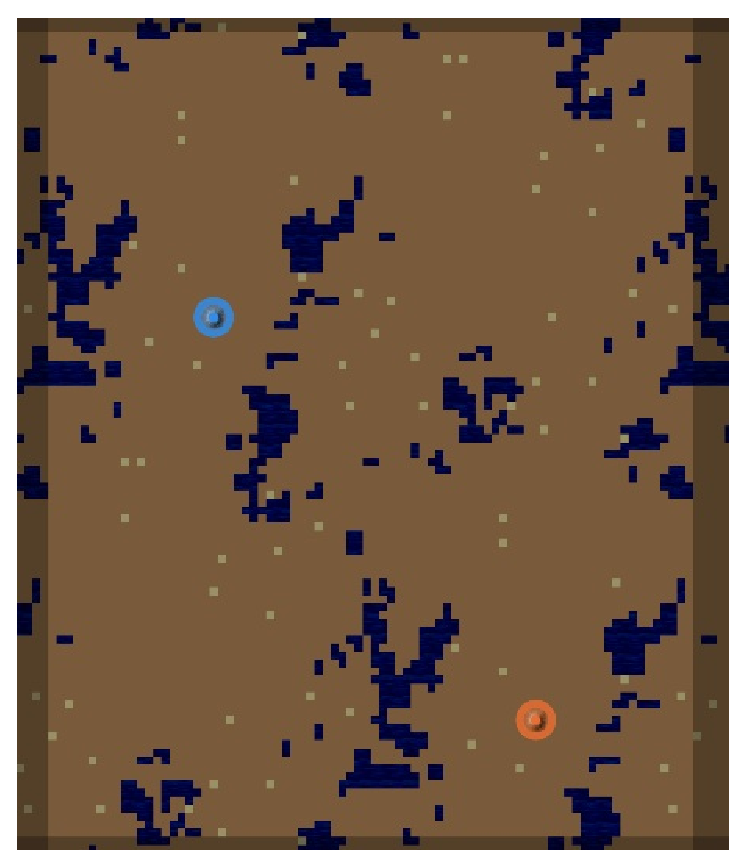
\includegraphics[scale =0.4] {images/map1.eps}
   \label{fig:subfig1}
 }
\subfigure[Map 3: maze/labyrinth type]{
   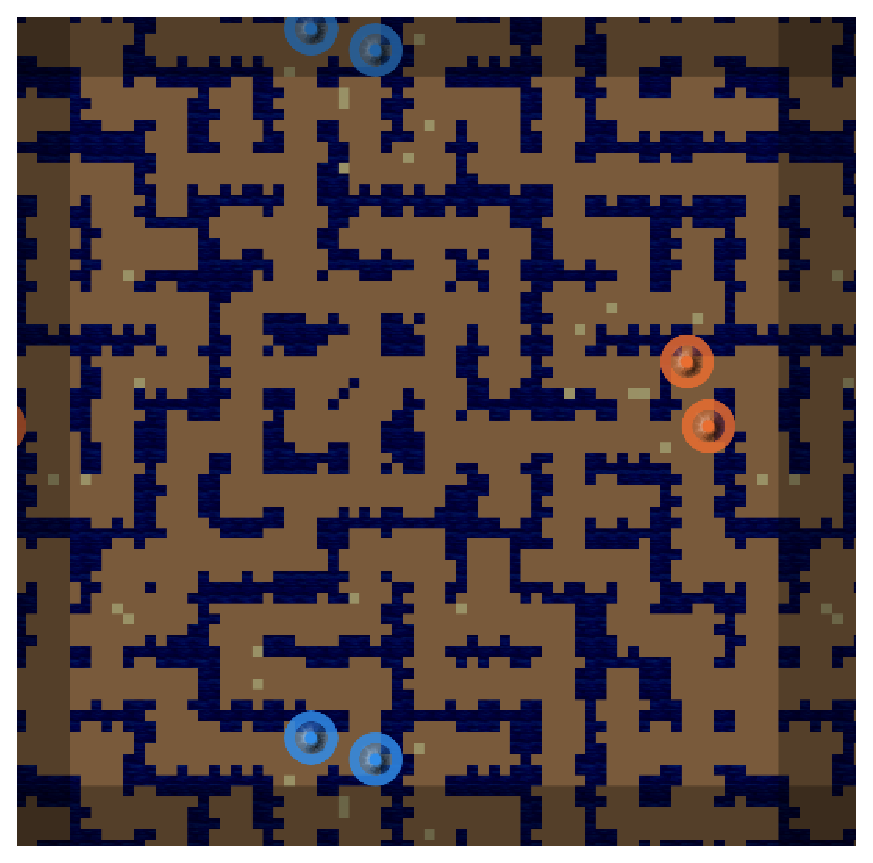
\includegraphics[scale =0.4] {images/map3.eps}
   \label{fig:subfig2}
 }
\label{fig:figmaps}
\caption{Two different example maps considered in the experiments. }
\end{figure}

In the experiments conducted it will be shown the performance of the implemented approaches (GA + fitness function) in each of the six previous maps. Both have considered an initial size of population of 64 individuals, a Crossover rate equal to 0.3, a mutation rate of 0.1 and a stop criterion set to 20 generations. Every agent is evolved in the six maps 10 times in order to get a feasible fitness value, trying to avoid the `noisy nature' \cite{Mora_noisy_jcst} of game playing to value an individual when the opponent is non-deterministic. I.e. the same agent could be valued as very good or very bad depending on the combat result, which in turn depends on the enemy's actions.

%%%%%%%%%%%%%%%%%%%%%%%%%%%%%%%%%%%%%%%%%%%%%%%%%%%%%%%%%%%%%%%%%%%%%%%%%%%%%%%

\section{Results and Analysis}
\label{sec:results}
% Table \ref{tab:basicfitness993} shows the fitness attained by the agent fith basic fitess calculator. 

% As can be seen...\textcolor{red}{ESTO TIENES QUE COMENTARLO. PON REFERENCIAS A LAS TABLAS}

Firstly it is important to notice that all the selected competitors got higher final rankings than our bot. Table \ref{tab:all} shows 


that our robot can not beat robots that are in positions 165 and 1. However, the evolution of the agent makes higher the number of own ants and decreases the number of enemy ants in a few generations. Genetic evolution of our agent wins on all maps to the robot that ended in ranking 993, more than 1000 position above the version without optimization. The number of ants is the main difference between basic fitness and hierarchical fitness, and this feature allows to use more effective attack techniques. In maps 5 and 6, the score is lower than the obtained with basic fitness in some cases. However, the number of ants own doubles to those obtained with a basic fitness. This invites us to improve strategies maps in such type of maps to achieve a better use of the large community of ants generated. A remarkable result is found in the standard deviation (SD) value. SD is zero in many cases because variables have very few possible values (i.e. in maps with only two hills, max\_score will be 0, 1 or 3 points) and after 20 generations the system evolves always to reach max score. 
%% Table generated by Excel2LaTeX from sheet 'fitness_only_score_vs_rank_993'
\begin{table}[htbp]
  \centering
  \caption{Results using basic fitness vs. Bot993. }
    \begin{tabular}{ccccc}
    \hline
          & \textbf{maxScore}  & \textbf{maxMyAnts}  & \textbf{maxEnemyAnts}   & \textbf{meanTurns}  \\
    \hline
    \textbf{map1} & 3,00  $\pm$ 0,00  & 84,08 $\pm$ 43,82 & 66,50 $\pm$ 49,20 & 416,87 $\pm$ 125,94 \\
    \textbf{map2} & 3,00  $\pm$ 0,00  & 68,08 $\pm$ 39,10 & 60,67 $\pm$ 34,92 & 425,64 $\pm$ 90,26 \\
    \textbf{map3}  & 6,00  $\pm$ 0,00  & 39,91 $\pm$ 15,65 & 186,91 $\pm$ 63,74 & 318,28 $\pm$ 124,63 \\
    \textbf{map4}  & 1,00  $\pm$ 0,00  & 8,64  $\pm$ 0,67  & 12,00 $\pm$ 0,00  & 150,00 $\pm$ 0,00 \\
    \textbf{map5} & 5,42  $\pm$ 0,51  & 36,00 $\pm$ 27,24 & 228,75 $\pm$ 89,91 & 428,93 $\pm$ 189,53 \\
    \textbf{map6} & 6,00  $\pm$ 0,00  & 46,25 $\pm$ 59,21 & 111,25 $\pm$ 20,82 & 221,18 $\pm$ 104,35 \\
   \hline 
   \end{tabular}%
  \label{tab:basicfitness}%
\end{table}%

%% Table generated by Excel2LaTeX from sheet 'fitness jerarquico vs rank993'

\begin{table}[htbp]
  \centering
  \caption{Results using hierarchical fitness vs. Bot993.}

    \begin{tabular}{ccccc}
    \hline
           & \textbf{maxScore} &   \textbf{maxMyAnts} &   \textbf{maxEnemyAnts} &\textbf{meanTurns}  \\
    \hline
    \textbf{map1} & 3,00  $\pm$ 0,00  & 154,56 $\pm$ 28,84 & 2,67  $\pm$ 1,50  & 481,33 $\pm$ 48,26 \\
    \textbf{map2} & 3,00  $\pm$ 0,00  & 97,67 $\pm$ 37,83 & 3,00  $\pm$ 2,18  & 486,78 $\pm$ 79,99 \\
    \textbf{map3} & 6,00  $\pm$ 0,00  & 45,00 $\pm$ 8,85  & 118,33 $\pm$ 19,49 & 266,00 $\pm$ 55,57 \\
    \textbf{map4} &  1,00  $\pm$ 0,00  & 9,22  $\pm$ 0,44  & 12,00 $\pm$ 0,00  & 150,00 $\pm$ 0,00 \\
    \textbf{map5} & 4,67  $\pm$ 0,50  & 73,78 $\pm$ 71,10 & 226,89 $\pm$ 57,61 & 706,78 $\pm$ 262,88 \\
    \textbf{map6} & 5,00  $\pm$ 1,15  & 104,11 $\pm$ 107,52 & 77,89 $\pm$ 58,10 & 519,44 $\pm$ 262,51 \\
    \hline
    \end{tabular}%

  \label{tab:hierarchical}%
\end{table}%

%% Table generated by Excel2LaTeX from sheet 'jerarquico_vs_player_165'
\begin{table}[htbp]
  \centering
  \caption{Results using hierarchical fitness vs. Bot165.}
    \begin{tabular}{ccccc}
    \hline
          & \textbf{maxScore} & \textbf{maxMyAnts} &  \textbf{maxEnemyAnts} &  \textbf{meanTurns}  \\
   \hline
    \textbf{map1} & 0,00  $\pm$ 0,00  & 33,58 $\pm$ 2,97  & 101,17 $\pm$ 7,83  & 183,42 $\pm$ 7,29 \\
    \textbf{map2} & 0,17  $\pm$ 0,39  & 31,08 $\pm$ 8,54  & 122,00 $\pm$ 49,41 & 221,17 $\pm$ 86,06 \\
    \textbf{map3} & 0,00  $\pm$ 0,00  & 35,33 $\pm$ 9,72  & 98,83 $\pm$ 10,99 & 186,50 $\pm$ 9,26 \\
    \textbf{map4} & 0,00  $\pm$ 0,00  & 34,75 $\pm$ 9,75  & 99,17 $\pm$ 10,96 & 184,92 $\pm$ 9,11 \\
    \textbf{map5} & 0,00  $\pm$ 0,00  & 32,50 $\pm$ 10,51 & 101,75 $\pm$ 12,19 & 186,25 $\pm$ 9,18 \\
    \textbf{map6} & 0,00  $\pm$ 0,00  & 31,50 $\pm$ 10,91 & 103,10 $\pm$ 12,80 & 188,00 $\pm$ 9,08 \\
    \hline
    \end{tabular}%
  \label{tab:addlabel}%
\end{table}%

%% Table generated by Excel2LaTeX from sheet 'jerarquico_vs_player_1'
\begin{table}[htbp]
  \centering
  \caption{Results using hierarchical fitness vs. Bot1.}
    \begin{tabular}{ccccc}
    \hline
          & \textbf{maxScore} & \textbf{maxMyAnts} &  \textbf{maxEnemyAnts} &  \textbf{meanTurns}  \\
   \hline
    \textbf{map1} & 0,00  $\pm$  0,00  & 31,00 $\pm$   34,00 & 109,00 $\pm$  95,00 & 185,00 $\pm$  198,00 \\
    \textbf{map2} & 0,00  $\pm$  0,00  & 17,00 $\pm$   23,00 & 119,00 $\pm$  132,00 & 156,00 $\pm$ 175,00 \\
    \textbf{map3} & 0,00  $\pm$  0,00  & 16,00 $\pm$   17,00 & 118,00 $\pm$  147,00 & 160,00 $\pm$ 186,00 \\
    \textbf{map4} & 0,00  $\pm$  0,00  & 14,00 $\pm$   17,00 & 130,00 $\pm$  120,00 & 166,00 $\pm$ 160,00 \\
    \textbf{map5} & 0,00  $\pm$  0,00  & 20,00 $\pm$   31,00 & 112,00 $\pm$  108,00 & 149,00 $\pm$ 147,00 \\
    \textbf{map6} & 0,00  $\pm$  0,00  & 21,00 $\pm$   19,00 & 127,00 $\pm$  131,00 & 172,00 $\pm$ 171,00 \\
    \hline
    \end{tabular}%
  \label{tab:addlabel}%
\end{table}%


\begin{table}[htbp]
  \centering
  \caption{Results}
    \begin{tabular}{ccccc}

    \hline
          & \textbf{maxScore}  & \textbf{maxMyAnts}  & \textbf{maxEnemyAnts}   & \textbf{meanTurns}  \\ 
    \hline
    \multicolumn{5}{c}{Basic fitness vs. Bot993.}\\ \hline
    \textbf{map1} & 3,00  $\pm$ 0,00  & 84,08 $\pm$ 43,82 & 66,50 $\pm$ 49,20 & 416,87 $\pm$ 125,94 \\
    \textbf{map2} & 3,00  $\pm$ 0,00  & 68,08 $\pm$ 39,10 & 60,67 $\pm$ 34,92 & 425,64 $\pm$ 90,26 \\
    \textbf{map3}  & 6,00  $\pm$ 0,00  & 39,91 $\pm$ 15,65 & 186,91 $\pm$ 63,74 & 318,28 $\pm$ 124,63 \\
    \textbf{map4}  & 1,00  $\pm$ 0,00  & 8,64  $\pm$ 0,67  & 12,00 $\pm$ 0,00  & 150,00 $\pm$ 0,00 \\
    \textbf{map5} & 5,42  $\pm$ 0,51  & 36,00 $\pm$ 27,24 & 228,75 $\pm$ 89,91 & 428,93 $\pm$ 189,53 \\
    \textbf{map6} & 6,00  $\pm$ 0,00  & 46,25 $\pm$ 59,21 & 111,25 $\pm$ 20,82 & 221,18 $\pm$ 104,35 \\
   \hline 
    \multicolumn{5}{c}{Hierarchical fitness vs. Bot993.}\\ \hline
    \textbf{map1} & 3,00  $\pm$ 0,00  & 154,56 $\pm$ 28,84 & 2,67  $\pm$ 1,50  & 481,33 $\pm$ 48,26 \\
    \textbf{map2} & 3,00  $\pm$ 0,00  & 97,67 $\pm$ 37,83 & 3,00  $\pm$ 2,18  & 486,78 $\pm$ 79,99 \\
    \textbf{map3} & 6,00  $\pm$ 0,00  & 45,00 $\pm$ 8,85  & 118,33 $\pm$ 19,49 & 266,00 $\pm$ 55,57 \\
    \textbf{map4} &  1,00  $\pm$ 0,00  & 9,22  $\pm$ 0,44  & 12,00 $\pm$ 0,00  & 150,00 $\pm$ 0,00 \\
    \textbf{map5} & 4,67  $\pm$ 0,50  & 73,78 $\pm$ 71,10 & 226,89 $\pm$ 57,61 & 706,78 $\pm$ 262,88 \\
    \textbf{map6} & 5,00  $\pm$ 1,15  & 104,11 $\pm$ 107,52 & 77,89 $\pm$ 58,10 & 519,44 $\pm$ 262,51 \\
    \hline
\multicolumn{5}{c}{Hierarchical fitness vs. Bot165.}\\ \hline
\textbf{map1} & 0,00  $\pm$ 0,00  & 33,58 $\pm$ 2,97  & 101,17 $\pm$ 7,83  & 183,42 $\pm$ 7,29 \\
    \textbf{map2} & 0,17  $\pm$ 0,39  & 31,08 $\pm$ 8,54  & 122,00 $\pm$ 49,41 & 221,17 $\pm$ 86,06 \\
    \textbf{map3} & 0,00  $\pm$ 0,00  & 35,33 $\pm$ 9,72  & 98,83 $\pm$ 10,99 & 186,50 $\pm$ 9,26 \\
    \textbf{map4} & 0,00  $\pm$ 0,00  & 34,75 $\pm$ 9,75  & 99,17 $\pm$ 10,96 & 184,92 $\pm$ 9,11 \\
    \textbf{map5} & 0,00  $\pm$ 0,00  & 32,50 $\pm$ 10,51 & 101,75 $\pm$ 12,19 & 186,25 $\pm$ 9,18 \\
    \textbf{map6} & 0,00  $\pm$ 0,00  & 31,50 $\pm$ 10,91 & 103,10 $\pm$ 12,80 & 188,00 $\pm$ 9,08 \\
\hline
\multicolumn{5}{c}{Hierarchical fitness vs. Bot1.}\\ \hline
    \textbf{map1} & 0,00  $\pm$  0,00  & 31,00 $\pm$   34,00 & 109,00 $\pm$  95,00 & 185,00 $\pm$  198,00 \\
    \textbf{map2} & 0,00  $\pm$  0,00  & 17,00 $\pm$   23,00 & 119,00 $\pm$  132,00 & 156,00 $\pm$ 175,00 \\
    \textbf{map3} & 0,00  $\pm$  0,00  & 16,00 $\pm$   17,00 & 118,00 $\pm$  147,00 & 160,00 $\pm$ 186,00 \\
    \textbf{map4} & 0,00  $\pm$  0,00  & 14,00 $\pm$   17,00 & 130,00 $\pm$  120,00 & 166,00 $\pm$ 160,00 \\
    \textbf{map5} & 0,00  $\pm$  0,00  & 20,00 $\pm$   31,00 & 112,00 $\pm$  108,00 & 149,00 $\pm$ 147,00 \\
    \textbf{map6} & 0,00  $\pm$  0,00  & 21,00 $\pm$   19,00 & 127,00 $\pm$  131,00 & 172,00 $\pm$ 171,00 \\
    \hline
   \end{tabular}%
  \label{tab:all}%
\end{table}%

% \textcolor{red}{Ojo, explicar por qué los mapas 4,5 y 6 el fitness jerárquico se comporta peor que el no jerárquico! Y por qué el minTurns es mayor de 150 en la mayoría?? Si tienes mucho lío escríbelo de forma entendible en español y luego lo traduzco yo si quieres. }

\section{Conclusions and future work}

This paper presents the design of an agent that plays in the RTS ANTS game proposed by Google AI Challenge. Starting with a combination of two basic behaviours (Lefty and Greedy) an Evolutionary Algorithm is used to set the parameters that modify the agent behaviour. This agent is evolved in the 6 maps provided by Google fighting three different bots that participated in the contest: the ones that finished in position 993, 165 and the winner. Results show that, even as evolving the parameters of two simple tasks, a fixed strategy agent is capable to win harder opponents. By the contrary, the same strategy is not affective against a middle bot, so it is clear that the enemy behaviour affects to the offline training algorithms with an specific strategy. Two different fitness functions have been tested: a basic function that only takes into account the final score (the number of conquered anthills in a run), and a hierarchical fitness, where the number of player's ants, turns, and enemy ants are also used to compare individuals. Genetic optimization is enough to beat a competitor who is above about 1000 positions in the ranking but, evolving a basic robot is not enough to beat robots with good strategies. We conclude that parameters optimization using GA significantly improves agent performance in RTS games and this technique obtains better results combined with good planning strategies.

 % \textcolor{red}{Results show that TERMINAR ESTO BIEN}
For future work, new combination of strategies will be studied and more different fitness will be analysed: for example, combining all maps in each fitness calculation. Because the stochastic behaviour of some robots also affects the fitness, an study of how this fitness is affected during the algorithm run will be performed. As demonstrated, the behaviour of the enemies is also a very important key to analyse for designing a all-terrain bot: an agent should adapt to these different behaviours. Also, using a quick map analysis in each turn to set the parameters obtained in this work could be studied to adapt the agent accordingly. A map analysis could be performed, for example, counting the number of
direction changes in a period of time. If many direction changes occurs by collisions with walls, means that bots are fighting in a map with maze pattern. Once map type has been detected, bot can choose suitable parameter group for the map. The combination of the Greedy and Lefty actions also will be studied in other RTS games, as the previous Google AI Contest games.

\bibliographystyle{plain}
\bibliography{botants}

\end{document}


